\documentclass[letter]{article}
\usepackage[monocolor]{../math232/ahsansabit}

\title{Quantum Mechanics Homework 01}
\author{Ahmed Saad Sabit, Rice University}
\date{\today}

\begin{document}
\maketitle

\section*{Problem 1 (a)}
\subsection*{\emph{Studying the problem}}
The initial configuration of the string 
\[
q(x,0) = f(x) = 
\begin{cases}
	\frac{2h}{L}x & 0 \le x \le \frac{L}{2} \\
	2h - \frac{2h}{L}x & \frac{L}{2} \le  x \le  L 
\end{cases}
\]
\[
	\frac{\partial q(x,t)}{\partial t} _{t=0} = \sum_{n=1}^{\infty} d_n \Omega_n \phi_n(x) = g(x) = 0 \implies \boxed{
	d_n = 0
	} 
\] 
The general solution to the string equation (assumed solution is separable between time and position)
\[
	q(x,t) = \sum_{n=1}^{\infty} [c_n \cos(\Omega_n t) + d_n \sin(\Omega_n t) ] \phi_n(x)
\]
For $t = 0$ we get, 
\[
	q(x,0) = f(x) = \sum_{n=1}^{\infty} c_n \phi_n(x)\] 
We are interested on finding the general solution of $q(x,t)$ that will hold for the future given this initial condition. The variables of our equation are obviously $x,t$ and what we need to find out is $c_n, d_n$. The next sub-section will find out a solution for $c_n$ ($d_n$ is trivially zero given zero initial velocity).



\subsection*{\emph{Solving for $c_n$} }
Let us do the following computation now. Let us multiply both sides of the above equation with $\phi_p(x)$ where $p$ represents the  $p$-th term while we take a summation over the index of $n$.
\[
f(x) \phi_p (x) = \sum_{n=1}^{\infty} c_n \phi_n(x) \phi_p(x)
\]
Just so that we can invoke the inner product between orthonormal bases, we can take an integral with the following way
\begin{align*}
	\int_{0}^{L} \mathrm{d} x \,  f(x) \phi_p(x) =& \int_{0}^{L} \mathrm{d} x\,  \left(
 \sum_{n=1}^{\infty} c_n \phi_n(x) \phi_p(x) \right) \\ 
		=& \sum_{n=1}^{\infty} c_n \int_{0}^{L} \mathrm{d} x \, \phi_n(x) \phi_p(x)  \\
		=& \sum_{n=1}^{\infty} c_n \delta_{np} \frac{L}{2} \\
		=& c_p \frac{L}{2}
\end{align*}
This above gives us the $p$-th term
\[
c_p = \frac{2}{L} \int_{0}^{L} \mathrm{d} x \, f(x) \phi_p(x) 
\] 
Using the explicit equation for the bases and also looking at the piecewise function, we can write, 
\begin{align*}
	c_p &= \frac{2}{L} \int_{0}^{L} \mathrm{d} x \, f(x) \sin \left( \frac{p \pi x }{L}\right)  \\
	&= \frac{2}{L} 
	\left( \int_{0}^{\frac{L}{2}}  f(x) \sin\left(\frac{p \pi x}{L}\right) + 
	\int_{\frac{L}{2}}^{L} f(x) \sin \left(\frac{p \pi x}{L}\right)  \right)\\
	&= \frac{2}{L} 
	\left(
	\int_{0}^{\frac{L}{2} } \frac{2h}{L} x \sin\left(\frac{p \pi x}{L}\right) +
	\int_{\frac{L}{2}}^{L} \left(2 h - \frac{2h}{L} x \right) \sin \left(\frac{p \pi x}{L}\right) 
	\right)\\
	&= 
	\frac{2}{L} 
	\left(
\frac{hL}{\pi ^2 p^2 } \left[ 
2 \sin \left(p \frac{\pi}{2} \right) - \pi p \cos \left(p \frac{\pi}{2}\right)
\right]  - \frac{hL}{\pi ^2 p ^2} 
\left[
	2 \sin\left(\pi p \right) - 2 \sin \left(p \frac{\pi}{2}\right) - \pi p \cos \left(p \frac{\pi}{ 2}\right)
\right]
	\right)\\ 
	&= \frac{8h}{\pi ^2 p^2} \sin \left(p \frac{\pi}{2}\right) \left[1 - \cos \left(p \frac{\pi}{2}\right)\right] \\
\end{align*}
Hence if I write this huge mess properly
\[
\boxed{
	c_n = \frac{8h}{\pi ^2 p ^2} \sin\left(\frac{p \pi }{2}\right) \left[ 1 - \cos \left(\frac{p \pi }{2}\right) \right]
}
\] 



\subsection*{\emph{Discussion on odd and even modes}}



\section*{Problem 1 (b)} 
\subsection*{\emph{Studying the Problem}}
Initially the string is tight and straight hence 
\[
q(x, 0) = \sum_{n=1}^{\infty} c_n \phi_n(x) = f(x) = 0 \implies \boxed{
c_n = 0
}
\] 
\[
	\frac{\partial q(x,t)}{\partial t} _{t = 0} = g(x) = v_0 \theta\left(a - \left|x - \frac{L}{2} \right|\right)
\]
Where $\theta(x)$ is a Heaviside step function (outputs 1 whenever input is 0 or positive).
I am not going to waste my and graders time by re-writing everything I wrote above, the procedure we are going to follow is same as above. 

\subsection*{\emph{Computation of $d_n$ }}
\begin{align*}
	g(x) &= \sum_{n=1}^{\infty} d_n \Omega_n \phi_n(x)   \\
\int_{0}^{L} \mathrm{d} x\, 	g(x) \phi_p (x) &= \sum_{n=1}^{\infty}  \int_{0}^{L} \mathrm{d} x \, d_n \Omega_n \phi_n (x) \phi_p (x)\\
\int_{L / 2 - a}^{L / 2  + a} v_0 \phi_p (x) &= d_p  \Omega_p \frac{L}{2}
\end{align*} 


\section*{Problem 3}
\begin{align*}
	| v + w | ^2 &=   \langle v + w | v + w \rangle  \\ 
	&= \langle v | v + w \rangle  + \langle w | v + w \rangle \\
	&=  \langle v | v \rangle + \langle v | w \rangle + 
	\langle w | v \rangle + \langle w | w \rangle \\ 
	&= | v | ^2 + | w | ^2 + \langle v| w \rangle + \langle v | w \rangle^* \\
	&= | v | ^2 + | w | ^2 + 2 \text{Re}\left( \langle v | w \rangle\right) \\
	&\le  |v|^2 + |w|^2 + 2 | \langle v | w \rangle |  \\
	&\le  |v|^2 + |w|^2 + 2 |v  | | w |  \\ 
	&\le \left( |v| + |w|\right)^2 \\
\end{align*}
This shows that 
\[
|v + w |  \le |v| + |w| 
\] 
\section*{Problem 4(a)}
I will write $\hat{\sigma}^{n}$ as simply $\sigma^{n}$ for this problem. I did the multiplication by hand. 
\[
	(\sigma^{1})^2 = 
	\begin{pmatrix} 0 & 1 \\ 1 & 0 \end{pmatrix} 
	\begin{pmatrix} 0 & 1 \\ 1 & 0 \end{pmatrix}  = 
	\begin{pmatrix} 1 & 0 \\ 0 & 1 \end{pmatrix} 
\] 

\[
	(\sigma^{2})^2 = 
	\begin{pmatrix} 0 & -i \\ i & 0 \end{pmatrix} 
	\begin{pmatrix} 0 & -i \\ i & 0 \end{pmatrix}  = 
	\begin{pmatrix} 1 & 0 \\ 0 & 1 \end{pmatrix} 
\]

\[
	(\sigma^{3})^2 =
	\begin{pmatrix} 1 & 0 \\ 0 & -1 \end{pmatrix} 
	\begin{pmatrix} 1 & 0 \\ 0 & -1 \end{pmatrix}  = 
	\begin{pmatrix} 1 & 0 \\ 0 & 1 \end{pmatrix} 
\]

We had been already defined 
\[
\sigma^{0} = 
	\begin{pmatrix} 1 & 0 \\ 0 & 1 \end{pmatrix} 
\] 

All of these result matrix above is the identity matrix that validates 
\[
	(\sigma ^{1})^2 = (\sigma ^{2})^2 = (\sigma ^{3})^2 = \sigma^0
\]



\section*{Problem 4(b)}
We are required to solve for $A^{\mu, \nu}$ where
\[
A^{\mu, \nu} = \sigma^{\mu} \sigma^{\nu} + \sigma^{\nu} \sigma^{\mu}
\] Note that it is obvious 
\[
A^{\mu, \nu} = A^{\nu , \mu}
\] 
Computing each of the matrix multiplications, and also referring to previous computations
\begin{align*}
	A^{k,k} = A^{1,1} = A^{2,2} = A^{3,3} = 2 (\sigma^{k})^2  = 2 \sigma^{0} = 
	2 \begin{pmatrix} 1 & 0 \\ 0 & 1 \end{pmatrix} 
\end{align*}
\begin{align*}
	A^{1,2} &=  
	\begin{pmatrix} 0 & 1 \\ 1 & 0 \end{pmatrix} 
	\begin{pmatrix} 0 & -i \\ i & 0 \end{pmatrix} 
+
	\begin{pmatrix} 0 & -i \\ i & 0 \end{pmatrix} 
	\begin{pmatrix} 0 & 1 \\ 1 & 0 \end{pmatrix}  \\ 
	&= 
	\begin{pmatrix} i & 0 \\ 0 & -i \end{pmatrix} + 
	\begin{pmatrix} -i & 0 \\ 0 & i \end{pmatrix} 
	\\	&=   \begin{pmatrix} 0 & 0 \\ 0 & 0 \end{pmatrix} 
\end{align*}

\begin{align*}
	A^{2,3} &= 
	\begin{pmatrix} 0 & -i \\ i & 0 \end{pmatrix} 
	\begin{pmatrix} 1 & 0 \\ 0 & -1 \end{pmatrix}  
+	\begin{pmatrix} 1 & 0 \\ 0 & -1 \end{pmatrix}  
	\begin{pmatrix} 0 & -i \\ i & 0 \end{pmatrix} 
	\\ 
			  &= \begin{pmatrix} 0 & i \\ i & 0 \end{pmatrix}  
	+ \begin{pmatrix}  0 & -i \\ -i & 0\end{pmatrix} 
			  \\
			     &= \begin{pmatrix} 0 & 0 \\ 0 & 0 \end{pmatrix}  \\
\end{align*}


\begin{align*}
	A^{1,3} &= 
	\begin{pmatrix} 0 & 1 \\ 1 & 0 \end{pmatrix} 
	\begin{pmatrix} 1 & 0 \\ 0 & -1 \end{pmatrix}  +
	\begin{pmatrix} 1 & 0 \\ 0 & -1 \end{pmatrix}  
	\begin{pmatrix} 0 & 1 \\ 1 & 0 \end{pmatrix}\\ &=
	\begin{pmatrix} 0 & -1 \\ 1 & 0 \end{pmatrix}  + 
	\begin{pmatrix} 0 & 1 \\ -1 & 0 \end{pmatrix}  \\ 
			  &= \begin{pmatrix} 0 & 0 \\ 0 & 0 \end{pmatrix}  
\end{align*}
Different indexes cause a zero-matrix, and similar causes a double of identity matrix. 
From here we can easily figure out that 
\[
	A^{\mu, \nu} = 2 \sigma^{0} \delta_{\mu, \nu}
\]

\section*{Problem 4(c)} 
I am going to borrow the computations I did last problem
\[
	\textsf{Tr} [ \sigma^{1 } \sigma ^{1} ] = 
	\textsf{Tr} \begin{pmatrix} 1 & 0 \\ 0 & 1  \end{pmatrix}  = 2
\] 
\[
	\textsf{Tr} [ \sigma^{2 } \sigma ^{2} ] = 
	\textsf{Tr} \begin{pmatrix} 1 & 0 \\ 0 & 1  \end{pmatrix}  = 2
\] 
\[
	\textsf{Tr} [ \sigma^{3 } \sigma ^{3} ] = 
	\textsf{Tr} \begin{pmatrix} 1 & 0 \\ 0 & 1  \end{pmatrix}  = 2
\] 

\[
	\textsf{Tr}[ \sigma^{1} \sigma^{2} ] = 
	\textsf{Tr} \begin{pmatrix} i&0\\0&-i \end{pmatrix} = 0
	= \textsf{Tr}[ \sigma^{2} \sigma^{1} ] 
\] 

\[
	\textsf{Tr}[ \sigma^{2} \sigma^{3} ] = 
	\textsf{Tr} \begin{pmatrix} 0&i\\i&0 \end{pmatrix} = 0
	= \textsf{Tr}[ \sigma^{3} \sigma^{2} ] 
\] 

\[
	\textsf{Tr}[ \sigma^{1} \sigma^{3} ] = 
	\textsf{Tr} \begin{pmatrix} 0&-1\\1&0 \end{pmatrix} = 0
	= \textsf{Tr}[ \sigma^{3} \sigma^{1} ] 
\] 

From this we can see that same-index gives $2$ and different gives 0. From this it's obvious
\[
	\textsf{Tr} [\sigma^{\mu} \sigma^{\nu} ] = 2 \delta_{\mu \nu}
\] 


\section*{Problem 4(d)}
Expanding the equation of the operator
\[
\hat{V} = \sum_{i = 1}^{3} V_i \sigma^{i} = V_1 \sigma^{1} + V_2 \sigma^{2} + V_3 \sigma^{3}
\]
Multiply $\sigma^{p}$ where $p \in \{1,2,3\} $ 
\[
\hat{V} \sigma^{p} = V_1 \sigma^{1} \sigma^{p} + V_2 \sigma^{2} \sigma^{p} + V_3 \sigma^{3} \sigma^{p}
\] 
Taking the trace and using the property $\textsf{Tr} (A + B) = \textsf{Tr} (A) + \textsf{Tr} (B)$  
\[
	\textsf{Tr} (\hat{V} \sigma^{p})  = 
	V_1 \left(2\delta_{1p}\right)+
	V_2 \left(2\delta_{2p}\right)+
	V_3 \left(2\delta_{3p}\right)
\]
From this using the definition of the $\delta_{\mu, p}$ we can simply write, 
\[
	V_p = \frac{1}{2} \textsf{Tr} (\hat{V} \sigma^{p})
\]
Using the form 
\[
	\hat{V} = \begin{pmatrix} a & b \\ c & d \end{pmatrix} 
\] we can find the coefficients $V_p$ 

\[
	\hat{V} \sigma^{0} = \begin{pmatrix} a & b \\ c & d \end{pmatrix} 
	\begin{pmatrix} 1 & 0 \\ 0 & 1 \end{pmatrix}  = 
	\begin{pmatrix} a & b \\ c & d \end{pmatrix}  \implies
	V_0 = \frac{a+d}{2}
\] 
\[
	\hat{V} \sigma^{1} = \begin{pmatrix} a & b \\ c & d \end{pmatrix} 
	\begin{pmatrix} 0 & 1 \\ 1 & 0 \end{pmatrix}  = 
	\begin{pmatrix} b & a \\ d & c \end{pmatrix}  \implies
	V_1 = \frac{b+c}{2}
\] 
\[
	\hat{V} \sigma^{2} = \begin{pmatrix} a & b \\ c & d \end{pmatrix} 
	\begin{pmatrix} 0 & -i \\ i & 0 \end{pmatrix}  = 
	\begin{pmatrix} ib & -ia  \\ id & -ic \end{pmatrix}  \implies
	V_2 = i\frac{b-c}{2}
\] 
\[
	\hat{V} \sigma^{3} = \begin{pmatrix} a & b \\ c & d \end{pmatrix} 
	\begin{pmatrix} 1 & 0 \\ 0 & -1 \end{pmatrix}  = 
	\begin{pmatrix} a & -b \\ c & -d \end{pmatrix}  \implies
	V_3 = \frac{a-d}{2}
\] 

So our representation is 
\[
	\begin{pmatrix} a & b \\ c & d \end{pmatrix}  = 
	\frac{a+d}{2}
	\begin{pmatrix} 1 &0 \\ 0 & 1\end{pmatrix}  + 
	\frac{b+c}{2} 
	\begin{pmatrix} 0 & 1 \\ 1 & 0 \end{pmatrix} +
	\frac{ib - ic}{2} 
	\begin{pmatrix} 0 & -i \\ i & 0 \end{pmatrix}  + 
	\frac{a-d}{2}
	\begin{pmatrix} 1 & 0 \\ 0 & -1 \end{pmatrix} 
\] 
I've checked this in Wolfram Alpha and it seems to work. 
\begin{figure}[htpb]
	\centering
	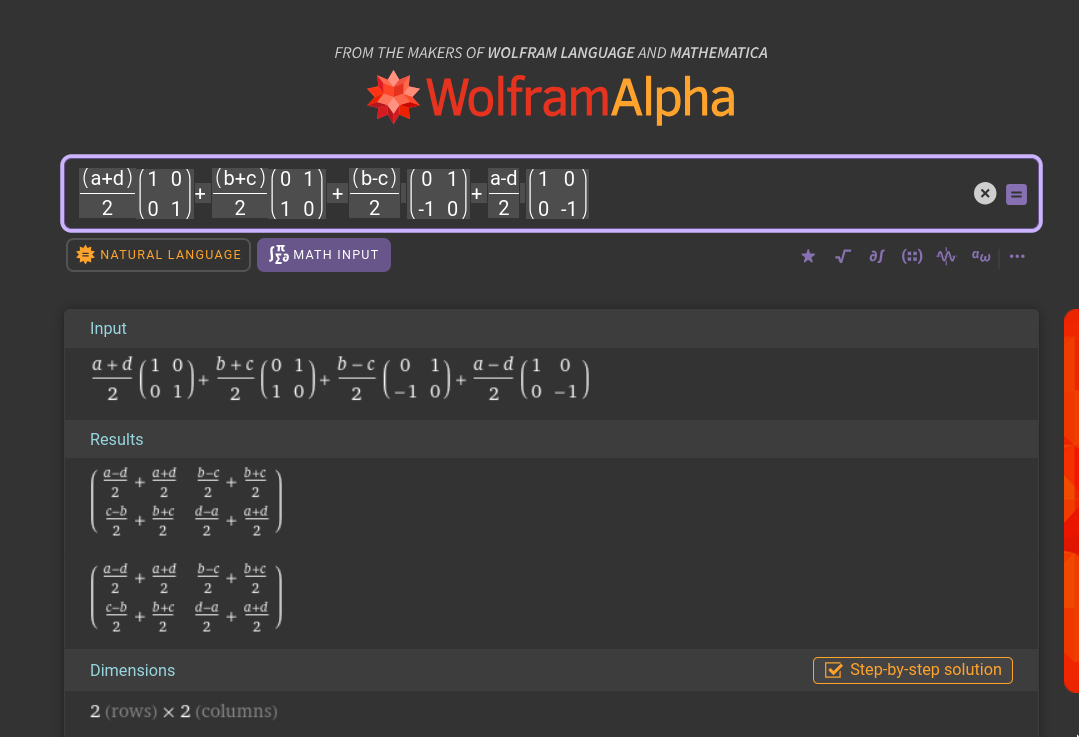
\includegraphics[width=0.8\textwidth]{ss/pauli-basis.png}
	\caption{ss/pauli-basis.png}
	\label{fig:ss-pauli-basis-png}
\end{figure}
\end{document}
